\documentclass[dvipdfmx]{jsarticle}
\usepackage[dvipdfmx]{graphicx}
\usepackage{amsmath, amssymb}
\usepackage{mathtools}
\usepackage{here}
\begin{document}
\title{週間進捗報告}
\author{権藤陸}
\maketitle
\section{進捗}
私事で恐縮ですが,外部院試の面接練習・対策に時間を割いていたため,進捗が少なめとなってしまっております.
情報工学輪講とFMCWレーダの研究室内発表が近いため,論文の読解を優先いたしました.

\begin{itemize}
    \item Sparsity Based Non-Contact Vital Signs Monitoring of Multiple People Via FMCW Radarの読解続き.中谷さんにお時間いただき,お話をして理解を深めました.
\end{itemize}

\section{論文の提案法}
先週との差分として,新しく理解できたこと,意味が明瞭になったと思われる部分をご報告いたします.理解が誤っている部分についてはご指摘いただけると幸いです.
\begin{figure}[htbp]
\begin{center}
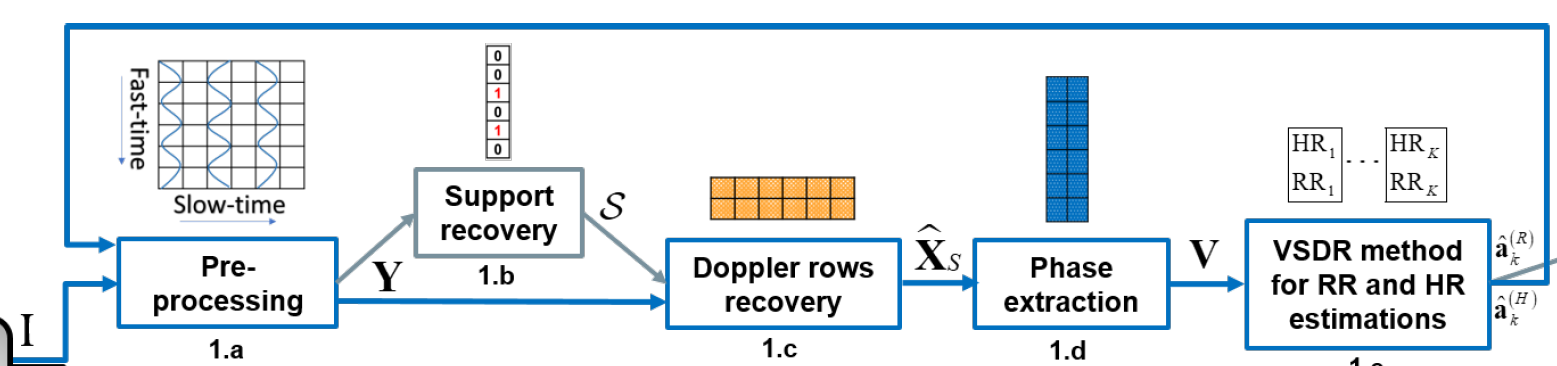
\includegraphics[width=\linewidth]{./img/NCVSM_diagram.png}
\end{center}
\caption{提案法の流れ[1]}
\end{figure}

\subsection{スパース性に基づく複数人に対する非接触な生体信号モニタリング}
\subsubsection{サポートリカバリーと人間位置推定}
\begin{equation}\label{}
\bar{\mathrm{Y}} = \frac{1}{L}(\mathrm{F^H_L} (\prod \odot \mathrm{F_L Y^T}))^T
\end{equation}

(1)式は,スペクトルフィルタリングを表しており,
$F_L$はL個のチャープフレームを含めた離散フーリエ変換行列で,FMCWレーダで測定した値が入っている$Y^T$を離散フーリエ変換し周波数領域に変換をしている.次に,$\prod$で表される通常時の呼吸と心拍の周波数帯に対応する窓関数で,通常の呼吸・心拍から外れる周波数帯の信号を切ってしまい,その後$F^H_L$で時間領域に戻している.

論文で言及されているJSR(Joint Sparse Recovery)技術とは一般的には,スパース性を活かした画像の欠損補完では,単一の画像(ベクトル)を用いて補完をするのに対し,(中谷さんから紹介していただいた)[2]のように,複数画像を用いて画像修復を行っていることを"Joint"と読んでいるので,本論文[1]においては,推定したい$\tilde{X}$がベクトルでなく行列のため,"Joint"であると理解しました.

\subsection{ドップラー行の復元}
以下の式で表される$\hat{\mathrm{X}_{\textit{S}}}$は,測定行列の$\mathrm{Y}$をslow-timeに沿ってフーリエ変換し,ドップラーの情報を得ている.
$\hat{\mathrm{X}}_{S}$は,サポート$S$に対応する行の推定真業行列,$\mathrm{F}_{S}$は離散フーリエ変換行列,Nはチャープの1フレーム内のサンプル数の2倍の定数,Yはレーダによる測定行列
その際にサポート$S$を用いることで,range-slowtimeマップ全体に対して計算を行う必要がないため効率的に計算が行える.

\begin{equation}\label{}
\mathrm{\hat{X}}_{S} = \frac{1}{N} \mathrm{F}_{S} \mathrm{Y}
\end{equation}

\subsection{位相抽出}
以下の式で,呼吸と心拍を推定するために$\hat{\mathrm{X}}_S$の近似値を抽出する.ここでもサポート$S$を用いることで人間のいる位置に対して位相推定が行えている.
\begin{equation}\label{}
V (l, k) \triangleq unwrap(\angle(\hat{\mathrm{X}}_{S}(S\{k\}, l)))
\end{equation}

式(3)のunwrap処理[3]とは位相補正のことであり,連続するサンプルの位相差を$\pi$未満にするために,$\pi$以上の位相変化に対しては,2$\pi$を加算または減算する処理である.位相差が$\pi$未満でなくてはならない理由は,隣り合うサンプルの位相差が$\pi$未満になるようなサンプリングレートを選択しているためである.
また,以下に文献[3]よりアルゴリズムと位相補正の図を掲載する.
\begin{figure}[H]
\begin{center}
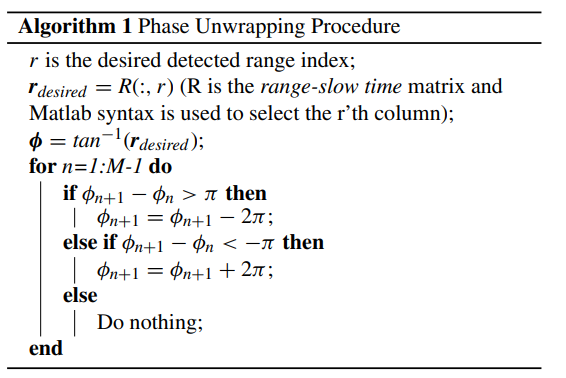
\includegraphics[width=0.8\linewidth]{./img/unwrap_2.png}
\end{center}
\caption{unwrapのアルゴリズム[3]}
\end{figure}

\begin{figure}[H]
\begin{center}
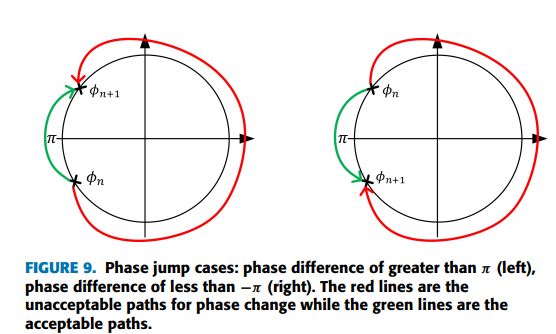
\includegraphics[width=0.8\linewidth]{./img/unwrap_1.png}
\end{center}
\caption{unwrapの模式図[3]}
\end{figure}

\subsection{呼吸数と心拍数を推定するための生体信号辞書に基づく復元}
人間の典型的な心拍と呼吸の周波数に基づく2つの辞書行列を用いて,心拍と呼吸を推定する.(4)式の行列$\mathrm{V}$は,検出された人間の胸壁変位を表す信号に対応するベクトルが$K$個並んだものである.
\begin{equation}\label{}
\mathrm{V} = [v_1, ..., v_K]
\end{equation}

$a_k^(R)を推定すべき呼吸信号の振幅,a_k^(H)を推定すべき心拍の振幅$として,各$v_k$は(5)式のように表される.$Dは呼吸と心拍周波数に関する辞書行列,n_kはノイズを表す列ベクトルである.$
辞書として周波数は用意したものから選択して,
\begin{equation}\label{}
v_k = D^(R) a_k^{(R)} + D^(H) a_k^{(H)} n_k
\end{equation}

そして,次の(6)式で推定を行う.
\begin{equation}\label{}
\hat{a}_k^{(R)} = D^{(R)T} v_k,\hat{a}_k^{(H)} = D^{(H)T} v_k
\end{equation}

\section{疑問点}
論文を読む中で分からなかった部分がありましたので,こちらにまとめさせていただきます.中谷さんと被る部分もあると思いますが,記載させていただきます.

\subsection{用語について}
\begin{itemize}
    \item ナイキストグリッド

    ナイキスト周波数のナイキストと格子を意味するグリッドが組み合わさり何を意味するかが分かりませんでした.レーダでサンプリングを行い離散値を取得しているのと,ナイキストの定理と関連があるのかと考えましたが,何を指しているのか不明です.

    \item サポート$\textit{S}$

サポート$\textit{S}$は,行座標と表現されていることと,図1にて0, 1の2値が要素となる列ベクトルであることが示唆されていること,一度計算した後は一連の提案法の流れの中で繰り返し同じ$\textit{S}$が用いられることから,人間のいる位置となる行には1が,人間のいない位置の行には0が入っており,その後の計算で1が入っている行については計算を行うために,インデックスとして用いられているのではないかと考えました.
\end{itemize}

\subsection{その他}
\begin{itemize}
    \item 式(1)の$F_L^H$は$F_L$の随伴行列であると思うのですが,この場合,逆離散フーリエ変換の処理を行うものであると理解してよろしいのでしょうか(計算結果が時間領域の値が要素の行列に見えます).
    \item 辞書的アプローチの推定である(6)式は,どのように導出されたのかが理解できていないです.(5)式から(6)式への変換が,かなり突拍子もない式変形のように見えます.$a_k$に非ゼロ要素を1つだけ持つベクトルであることが特徴的なので,それを利用しているのかなどと考えています.
\end{itemize}

\section{計画}
\begin{itemize}
    \item 論文[1]の読解とプレゼン準備
    \item レンジドップラーマップの実装
    \item 情報工学輪講の準備
\end{itemize}


\begin{thebibliography}{}
\item Yonathan Eder, \textit{Graduate Student Member, IEEE, }and Yonina C. Eldar, \textit{Fellow, IEEE}, "Sparsity Based Non-Contact Vital Signs Monitoring of Multiple People Via FMCW Radar", arXiv:, 2205.05152v1 [eess.SP], 10 May 2022
\item U. Rossman, R. Tenne, O. Solomon, I. Kaplan-Ashiri, T. Dadosh, Y. C. Eldar, and, D. Oron,
“ Rapid quantum image scanning microscopy by joint sparse reconstruction, ” Optica, vol. 6,
no. 10, pp. 1290–1296, 2019.
\item  M. Alizadeh, G. Shaker, J. C. M. D. Almeida, P. P. Morita and S. Safavi-Naeini, "Remote Monitoring of Human Vital Signs Using mm-Wave FMCW Radar," in IEEE Access, vol. 7, pp. 54958-54968, 2019, doi: 10.1109/ACCESS.2019.2912956.
\end{thebibliography}
\end{document}